\subsection{Behavior directions transfer before generation on some datasets}
\label{sec:results-behavior}

We test whether contrastive directions extracted from answers predict behavior before generation. Following \citet{chen2025personavectors}, we extract fixed answer and context directions, $v_A$ and $v_C$, from positive-minus-negative instruction contrasts for harmful compliance (including malicious persona and style), sycophancy, and hallucination. With a frozen layer-19 metamodel trained on 963,444 generic pairs, we compare three projections: the answer direction on predicted answers ($v_A^\top\hat h_A$), the same direction on observed answers ($v_A^\top\bar h_A$), and the context direction on contexts ($v_C^\top h_C$). We evaluate Spearman correlation with mean retained behavior scores per context on five held-out datasets (\appref{app:behavior}).

\noindent\textbf{Transferred answer directions do not consistently outperform context directions} (\figref[A]{fig:behavior-prediction})\textbf{:} Projecting predicted answers onto the answer direction gives $\rho=0.426$, 0.255, and 0.449 on ToxicChat, AITA, and SimpleQA, compared with 0.403, 0.319, and 0.507 for context directions. The same answer directions on observed answers give 0.440, 0.215, and 0.605, validating the answer-side association on these datasets. Transfer improves on the context direction on HH-RLHF (0.058 versus 0.001), but remains weak. Both methods are negatively correlated on NQ-Open, where even the observed-answer direction fails validation ($\rho=-0.009$).

\noindent\textbf{Preimages do not consistently outperform context directions} (\figref[B]{fig:behavior-prediction})\textbf{:} A regularized inverse finds a context direction that the metamodel's linear component maps approximately onto the fixed answer direction. Preimage scores are close to context-native scores on ToxicChat (0.410 versus 0.403) and AITA (0.322 versus 0.319), but lower on SimpleQA (0.435 versus 0.507). Prediction remains weak on HH-RLHF ($\rho=0.051$) and reverses on NQ-Open ($-0.171$).

\noindent\textbf{Preimage retrieval reveals recurring prompt types} (\tabref{tab:behavior-preimage-examples})\textbf{:} The nearest generic contexts include malicious-persona requests, benign interpersonal-response prompts, and detailed chemical-company introductions. All 30 highest-ranked hallucination contexts share the company-introduction template. These unjudged training-pool examples show semantic associations, but do not establish that the prompts induce the intended behavior.

% Sources: EPS eval_results/issue_1739/million_cached_20260916.
% Renderer: scripts/issue1739_behavior_paper_figures.py, hash-checked summaries.
\begin{figure*}[t]
    \centering
    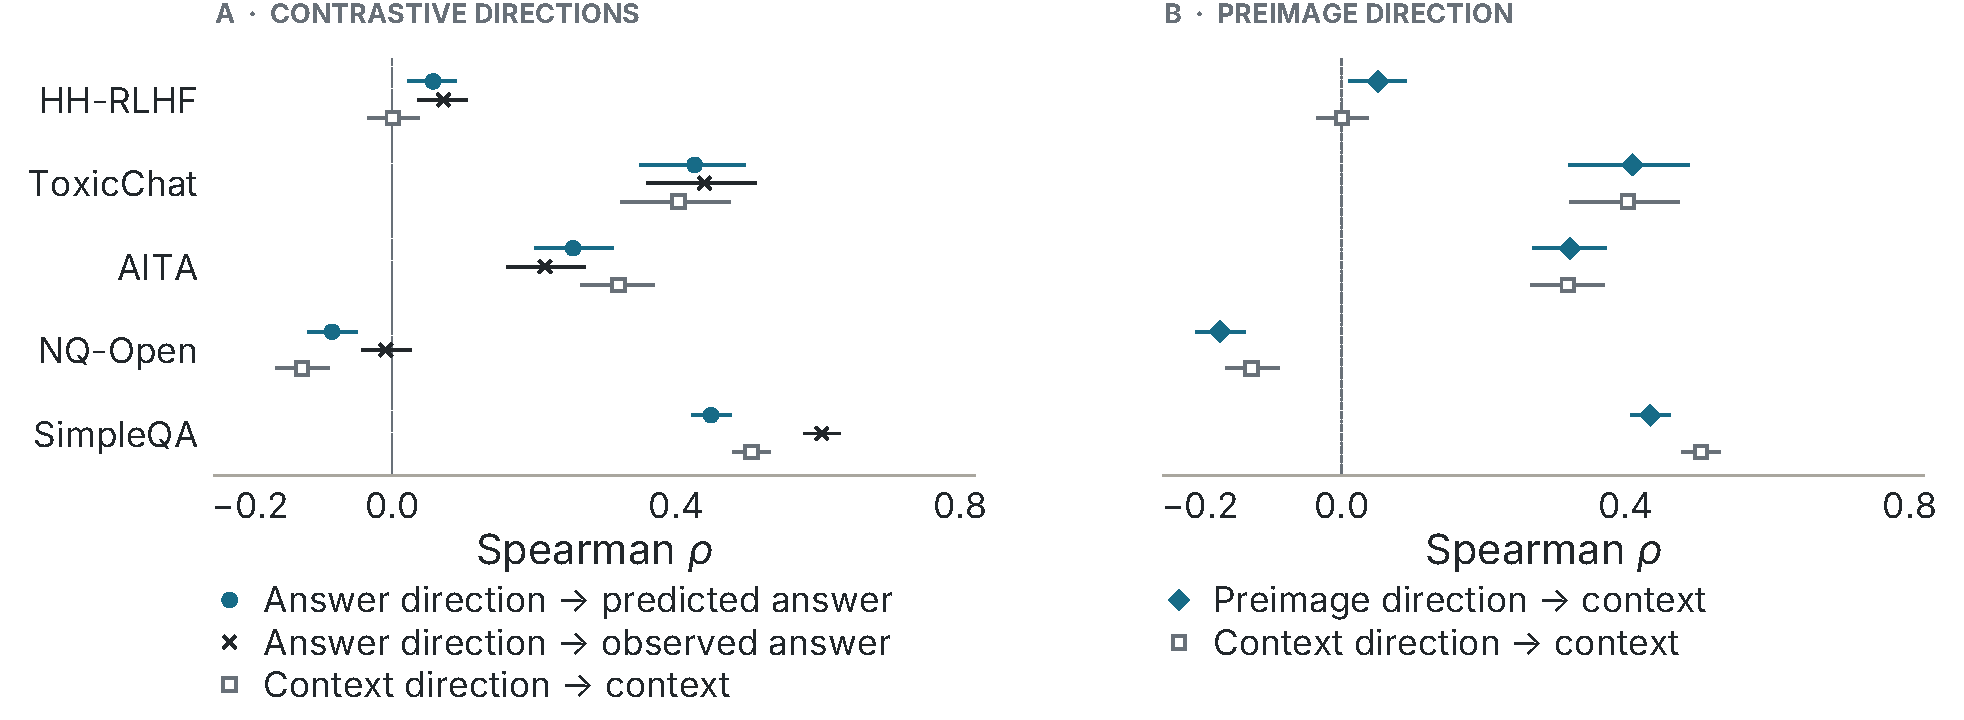
\includegraphics[width=\textwidth]{figures/paper/c5_behavior_transfer.pdf}
    \caption{\panel{A} \textbf{Transferred answer directions do not consistently outperform context directions.} The same contrastive answer direction scores predicted and observed answers, compared with a contrastive context direction scoring contexts.
    \panel{B} \textbf{Preimages do not consistently outperform context directions.} Regularized inverse directions versus contrastive context directions. All directions are fixed before evaluation.
    HH-RLHF and ToxicChat score harmful compliance including malicious persona and style, AITA sycophancy, and NQ-Open and SimpleQA hallucination. Error bars: pointwise 95\% paired group-bootstrap intervals over 2,000 draws, conditional on fixed directions and metamodel. Qwen2.5-7B-Instruct, layer 19, 963,444 training pairs.
    Details: \appref{app:behavior}.}
    \label{fig:behavior-prediction}
\end{figure*}
